\documentclass[reprint,english,notitlepage,nofootinbib]{revtex4-1}  % defines the basic parameters of the document
% if you want a single-column, remove reprint

% allows special characters (including æøå)
\usepackage[utf8]{inputenc}
% \usepackage [norsk]{babel} %if you write norwegian
\usepackage[english]{babel}  %if you write english


\usepackage{makecell}       %denne gjør at man kan ha nye linjer

\usepackage{physics,amssymb}  % mathematical symbols (physics imports amsmath)
\usepackage{graphicx}         % include graphics such as plots
\usepackage{xcolor}           % set colors
\usepackage{hyperref}         % automagic cross-referencing (this is GODLIKE)
\usepackage{tikz}             % draw figures manually
\usepackage{listings}         % display code
\usepackage{subfigure}        % imports a lot of cool and useful figure commands

% defines the color of hyperref objects
% Blending two colors:  blue!80!black  =  80% blue and 20% black
\hypersetup{ % this is just my personal choice, feel free to change things
    colorlinks,
    linkcolor={red!50!black},
    citecolor={blue!50!black},
    urlcolor={blue!80!black}}

%% Defines the style of the programming listing
%% This is actually my personal template, go ahead and change stuff if you want
\lstset{ %
	inputpath=,
	backgroundcolor=\color{white!88!black},
	basicstyle={\ttfamily\scriptsize},
	commentstyle=\color{magenta},
	language=Python,
	morekeywords={True,False},
	tabsize=4,
	stringstyle=\color{green!55!black},
	frame=single,
	keywordstyle=\color{blue},
	showstringspaces=false,
	columns=fullflexible,
	keepspaces=true}


\begin{document}


\title{FYS3150 - Project 2}
\date{\today}
\author{Vegard Falmår and Sigurd Sørlie Rustad}
\affiliation{Universitetet i Oslo}

\email{vegardfa@uio.no}
\email{sigurdsr@gmail.com}
\newpage

\begin{abstract}

\end{abstract}
\maketitle


\section{Introduction}

The harmonic oscillator (HO) potential appears in many areas within quantum physics. This is because many potentials can be approximated, at least in some intervals, with a HO potential. The most famous example of this might be the model for a hydrogen atom, where the electron is bound to the proton by a HO potential. That is why, in this report, we are going to study both one and multiple electrons in a HO potential. We are also going to account for electrical forces between the particles.

When we try to solve Schrodinger's equation for both one and two particles, we end up with a eigenvalue problem (see theory section). This can be represented with a linear set of equations written on matrix-form (a derivation can be found in our project 1\footnote{github.com/sigurdru/FYS3150/blob/master/Project1/tex/Project1.pdf}). Using Jacobi's rotation algorithm, also described in the theory section, we can diagonalize the matrix to find these eigenvalues and eigenvectors. Then plot the results, comparing them to experimental values.

When implementing algorithms it is important to test your code and make sure it performs as expected. Therefore we perform unit-tests to make sure sections of our program works as expected. We also test the code with a test scenario (buckling beam), which have analytical eigenvalues and eigenvectors. The testing is described in the appendix (\ref{appendix}).

For our studies we have used c++ for heavy computation, python for visualization and bash for automation. All the code along with instructions on how to run it, can be cloned from our GitHub repository here\footnote{github.com/sigurdru/FYS3150/tree/master/Project2}.


\section{Theory}

\subsection{Unitary transformation}
The transposed of a unitary matrix ($U$) is its inverse.
\begin{equation*}
	U^T = U^{-1}
\end{equation*}
From this we can prove that a unitary transformation preserves the orthonormality of vectors. Consider the set of orthonormal vectors $\{ \mathbf{v}_i \}_i$ and the unitary transformation $\{ U\mathbf{v}_i \}_i = \{ \mathbf{w}_i \}_i$.
\begin{align*}
	\mathbf{w}_i^T\mathbf{w}_j &= (U\mathbf{v}_i)^TU\mathbf{v}_j \\
	&= \mathbf{v}_i^TU^TU\mathbf{v}_j = \mathbf{v}_i^T\mathbf{v}_j \\
	&= \delta_{i,j}
\end{align*}
We notice that orthonormality is perserved.

\subsection{Jacobi's rotation algorithm}
Jacobi's rotation algorithm uses unitary transformations to diagonalize a matrix. A detailed description of the algorithm can be found here \citep{lecnotes}, however we will describe it briefly. In order to diagonalize a given matrix $A$, as mentioned over, we perform a series of unitary transformations.
\begin{equation*}
	B = U_n^T U_{n-1}^T ... U_0^T A U_0 ... U_{n-1}U_n
\end{equation*}
Here $U_i$ are the unitary matrices and $B$ the resulting diagonal matrix. An example of how $U_i$ can look is given under.
\begin{equation*}
	  \begin{bmatrix}
	1  & 0 & ...  & 0 & 0 & ... & 0 & 0 \\
	0 & 1  & ... & 0 & 0 & ... & 0 & 0 \\
	...  & ... & ... & ... & ... & ... & 0 & ... \\
	0  & 0 & ... & \cos \theta & 0 & ... & 0 & \sin \theta \\
	0  & 0 & ... & 0 & 1 & ... & 0 & 0 \\
	...  & ...& ...  &... & ...   & ... &1 &...  \\
	0  & 0& ...  & -\sin \theta &0 & ... &0 &\cos \theta  \\
	\end{bmatrix}
\end{equation*}
The geometric interpretation is that $U_i$ performs a rotation on $T$ in order to zero out non-diagonal elements. It turns out that the fastest way to do this, is to zero out the largest non-diagonal matrix-element. First We define:
\begin{equation*}
	\cot(\theta) = \tau = \frac{a_{ll} - a_{kk}}{2a_{kl}},
\end{equation*}
Where $a_{kl}$ is the largest non-diagonal element in $A$. Now to shorten notation we use $\tan(\theta) = t = s/c$, where $s = \sin(\theta) \wedge c = \cos(\theta)$. By defining $\theta$ such that $a_{kl}$ becomes zero we get the quadratic equation
\begin{equation*}
	t^2 + 2\tau t -1 = 0 \implies t = -\tau \pm \sqrt{1+\tau^2},
\end{equation*}
and can also obtain $c$ and $s$
\begin{equation*}
	c = \frac{1}{1+t^2} \wedge s = tc.
\end{equation*}
The actual transformation is defined by the set of equations
\begin{align}
\begin{split}
	b_{ik} &= a_{ik}c - a_{il}s, i \neq k, i \neq l \\
	b_{il} &= a_{il}c + a_{ik}s, i \neq k, i \neq l \\
	b_{kk} &= a_{kk}c^2 - 2a_{kl}cs + a_{ll}s^2 \\
	b_{ll} &= a_{ll}c^2 + 2a_{kl}cs + a_{kk}s^2 \\
	b_{kl} &= (a_{kk} - a_{ll} )cs + a_{kl}(c^2 - s^2)
	\label{eq:jacobi}
\end{split}
\end{align}
Where $b_{ij}$ are elements in $B$, again see \citep{lecnotes} for a more detailed description of the algorithm.

An interesting question is; what happens to the eigenvectors and eigenvalues? Because $B$ is diagonal the eigenvectors are just vectors with a $1$ in one element and $0$ everywhere else. We consider an arbitrary eigenvector $\mathbf{v}$ and eigenvalue $\lambda$ that satisfy
\begin{equation*}
	B\mathbf{v} = \lambda \mathbf{v} .
\end{equation*}
Applying the unitary transforms we get
\begin{align*}
	B\mathbf{v} &= U_n^T U_{n-1}^T ... U_0^T A U_0 ... U_{n-1}U_n \mathbf{v} \\
	&= \lambda \mathbf{v} \\
 \end{align*}
We notice that this is true if
\begin{equation}
	\mathbf{v'} = U_0 ... U_{n-1}U_n \mathbf{v}
	\label{eq:vmark}
\end{equation}
is an eigenvector with eigenvalue $\lambda$ that satisfy
\begin{equation*}
	A \mathbf{v}' = \lambda \mathbf{v}'
\end{equation*}
Therefore, if you have the eigenvector $\mathbf{v}$ and matrices $U_i$ you can find $\mathbf{v}'$ with equation (\ref{eq:vmark}).

\subsection{Electrons in a harmonic oscillator potential}

It turns out that if you try to solve Schrodinger's equation you end up with a eigenvalue problem. We will derive the math here, but everything is taken from here \citep{oppgavetekst}. First we consider the Schrodinger's equation for one electron. Because of spherical symmetry we only need to look at the radial part.
\begin{equation}
	-\frac{\hbar^2}{2m}\bigg(\frac{1}{r^2}\frac{d}{dr}r^2\frac{d}{dr}-\frac{l(l+1)}{r^2}\bigg)R(r) + V(r) R(r) = ER(r)
	\label{eq:SE}
\end{equation}
Where $R(r)$ is the radial wave equation, $V(r)$ the potential, $l$ orbital momentum and $r$ distance from the origin. Now because we only have one electron we end up with the HO potential $V(r) = (1/2)kr^2$. Substituting $R(r) = (1/r)u(r)$ and $\rho = (1/\alpha)r$ (where $\alpha$ is a constant with dimension length) we obtain
\begin{equation*}
	-\frac{\hbar^2}{2m\alpha^2}\frac{d^2}{d\rho^2}u(\rho) + \left(V(\rho) + \frac{l(l+1)}{\rho^2}\frac{\hbar^2}{2m\alpha^2}\right)u(\rho) = Eu(\rho).
\end{equation*}
Setting the orbital momentum $l=0$, inserting $V(\rho) = (1/2)k\alpha^2\rho^2$ and defining
\begin{equation*}
	\alpha \equiv \left(\frac{\hbar^2}{mk}\right)^{1/4} \wedge \lambda \equiv \frac{2m\alpha^2}{\hbar}E
\end{equation*}
Schrodinger's equation can then be described by the simple equation (\ref{eq:SE1}).
\begin{equation}
	-\frac{d^2}{d\rho^2}u(\rho)+\rho^2u(\rho) = \lambda u(\rho)
	\label{eq:SE1}
\end{equation}
Now we can expand our model to two particles with Coulomb potential between them. First introducing the relative position $\mathbf{r}$ and center-of-mass coordinate $\mathbf{R}$
\begin{equation*}
	\mathbf{r} = \mathbf{r_1} - \mathbf{r_2} \wedge \mathbf{R} = \frac{1}{2(\mathbf{r_1}+\mathbf{r_2})}.
\end{equation*}
Where $\mathbf{r_1}$ and $\mathbf{r_2}$ are the particles positions.Then the radial Schrodinger's becomes
\begin{equation*}
	\left(  -\frac{\hbar^2}{m} \frac{d^2}{dr^2} -\frac{\hbar^2}{4 m} \frac{d^2}{dR^2}+ \frac{1}{4} k r^2+  kR^2\right)u(r,R)  = E^{(2)} u(r,R).
\end{equation*}
$E^{(2)}$ denotes the fact that we are looking at the total energy of two particles. From an ansatz for the wave equation, we can perform separation of variable on $r$ and $R$.
\begin{equation*}
	u(r, R) = \psi(r)\phi(R) \wedge E^{(2)} = E_r + E_R
\end{equation*}
Adding the Coulomb potential
\begin{equation*}
	\frac{\beta e^2}{r}
\end{equation*}
between the two electrons we get
\begin{equation*}
	\left(  -\frac{\hbar^2}{m} \frac{d^2}{dr^2}+ \frac{1}{4}k r^2+\frac{\beta e^2}{r}\right)\psi(r)  = E_r \psi(r).
\end{equation*}
Again introducing $\rho = r/\alpha$ and defining a few variables
\begin{equation*}
	\omega_r^2\equiv \frac{1}{4}\frac{mk}{\hbar^2} \alpha^4 \wedge \alpha \equiv \frac{\hbar^2}{m\beta e^2} \wedge \lambda \equiv \frac{m\alpha^2}{\hbar^2}E
\end{equation*}
We arrive at the Schrodinger's equation (\ref{eq:SE2})
\begin{equation}
	-\frac{d^2}{d\rho^2}\psi(\rho) + \omega_r^2\rho^2\psi(\rho) + \frac{1}{\rho}\psi(\rho) = \lambda\psi(\rho)
	\label{eq:SE2}
\end{equation}

\section{Method}

As mentioned in the theory section, when you study one or more particles in a HO potential, you get a eigenvalue problem. For one particle this is given by equation (\ref{eq:SE1}). From Project 1 (see the theory section from Project 1\footnote{github.com/sigurdru/FYS3150/blob/master/Project1/tex/Project1.pdf}) we know this type of differential equation creates a set of equations, that can be represented as follows.
\begin{equation}
  \label{eq:discrete_2nd_deriv_mat}
	\scriptsize{\begin{bmatrix}d_1 & e_1 & 0   & 0    & \dots  &0     & 0 \\
		e_1 & d_2 & e_2 & 0    & \dots  &0     &0 \\
		0   & e_2 & d_3 & e_3  &0       &\dots & 0\\
		\dots  & \dots & \dots & \dots  &\dots      &\dots & \dots\\
		0   & \dots & \dots & \dots  &  e_{N-3}     &d_{N-2} & e_{N-2}\\
		0   & \dots & \dots & \dots  &\dots       &e_{N-2} & d_{N-1}
	\end{bmatrix}  \begin{bmatrix} u_{1} \\
		u_{2} \\
		\dots\\ \dots\\ \dots\\
		u_{N-1}
	\end{bmatrix}=\lambda \begin{bmatrix} u_{1} \\
		u_{2} \\
		\dots\\ \dots\\ \dots\\
		u_{N-1}
  \end{bmatrix}}
\end{equation}
Where $e_i = -1/h^2$, $d_i = 2/h^2 + V_i$ and $h = (\rho_N - \rho_0)/N$. $\rho_0$ and $\rho_N$ are the endpoints that in reality goes from $\rho_0 = 0$ to $\rho_N=\infty$. Of course we cannot do this for $\rho_N = \infty$, so we have to decide on a maximum we want to evaluate. We do this with trial end error. Our other problem is to decide the number of integration points $N$. As with the endpoint $\rho_N$ we try for different values and interpret the solutions.

We can solve this with Jacobi's rotation algorithm described in the theory section. In order to do this we use the sets of equations (\ref{eq:jacobi}). To make sure algorithm was implemented properly we performed several tests. First unit-tests to make sure small chunks run as expected, then with a buckling beam problem that has analytical eigenvalues and eigenvectors. Further information on the tests can be found in the appendix (\ref{appendix}).


\section{Results}

\begin{figure}[h]
	\centering
	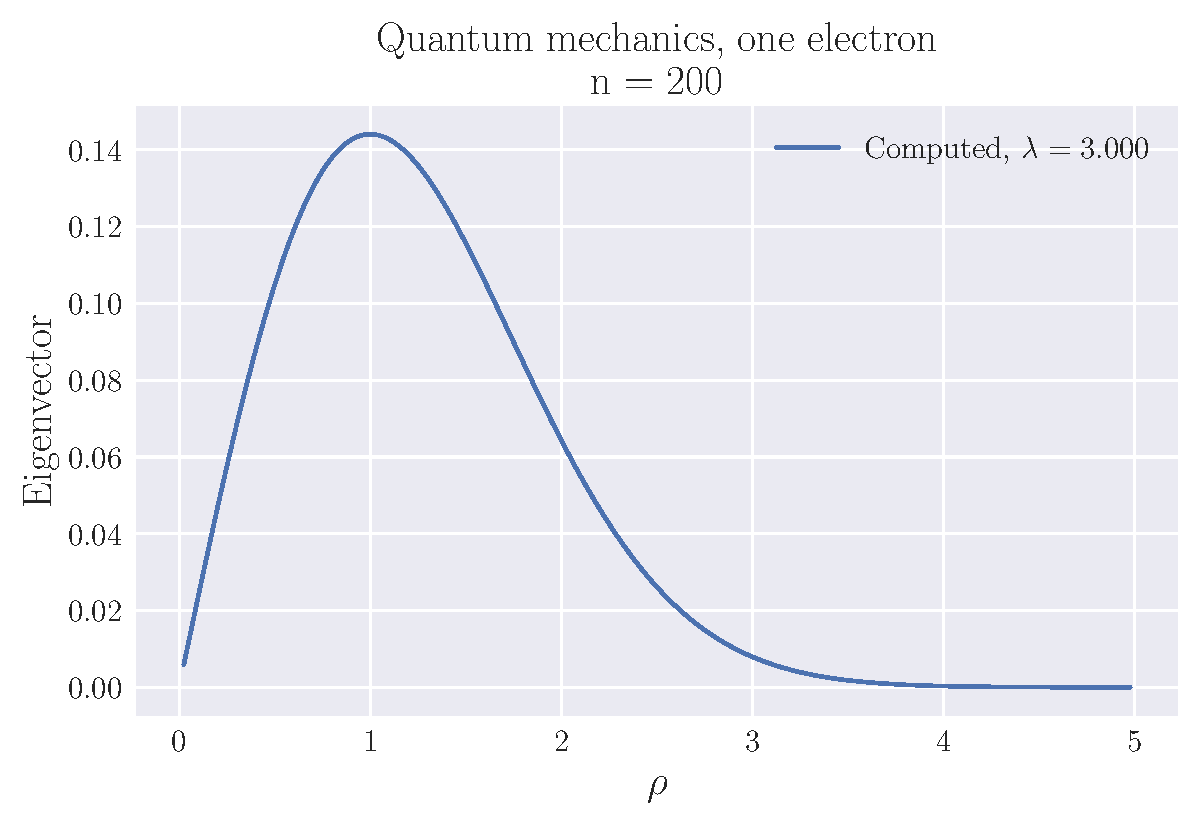
\includegraphics[width=\linewidth]{../output/QM1_200_0.pdf}
	\label{fig:QM200}
	\caption{}
\end{figure}


\begin{figure}[h]
	\centering
	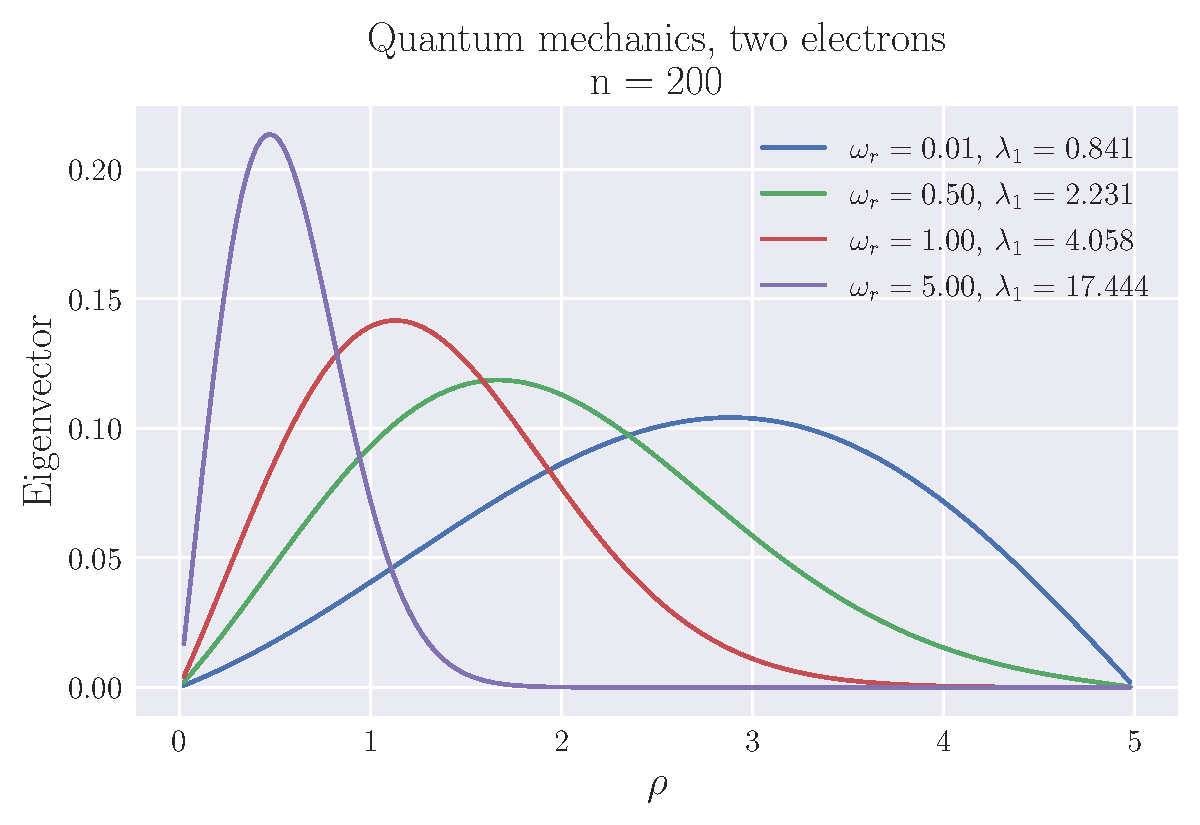
\includegraphics[width=\linewidth]{../output/QM2_200.pdf}
	\label{fig:QM2002}
	\caption{}
\end{figure}

\section{Discussion}

\section{Conclusion}

\section{Appendix}
\label{appendix}

\subsection{Buckling beam}

The simplest use case for our algorithm is a second order differential equation like \ref{eq:SE1} and \ref{eq:SE2}, but without the potential. One such example is equation \ref{eq:BB} for the vertical displacement $u(\rho)$ of a horisontal beam of length $L$ when a force is applied in the x-direction towards the origin. $\rho = x/L \in [0, 1]$, where $L$ is the length of the beam, is a dimensionless length. The constant $\lambda$ can be expressed as $\lambda = F L^2 / \gamma$, where $F$ is the applied force and $\gamma$ is a constant defined by properties like the rigidity of the beam.
\begin{equation}
	-\frac{d^2}{d\rho^2}u(\rho) = \lambda u(\rho)
	\label{eq:BB}
\end{equation}

Discretizing this equation gives a matrix equation on the form of equation \ref{eq:discrete_2nd_deriv_mat} with $e_i = e = -1/h^2$ and $d_i = d = 2/h^2$, where $h$ again is the step size. This is a tridiagonal Toeplitz matrix which has analytical eigenvalues described by \ref{eq:BB_eigvals} and analytical eigenvectors described by \ref{eq:BB_eigvecs}, both for $j = 1, 2, ..., N-1$.
\begin{align}
  \lambda_j &= d + 2 e \cos{\left( \frac{j \pi}{N} \right)} \label{eq:BB_eigvals} \\
  \mathbf u_j &= \left[ \sin{\left( \frac{j \pi}{N} \right)}, \sin{\left( \frac{2 j \pi}{N} \right)}, ..., \sin{\left( \frac{(N-1) j \pi}{N} \right)} \right]^T \label{eq:BB_eigvecs}
\end{align}

\begin{figure}[h]
	\centering
	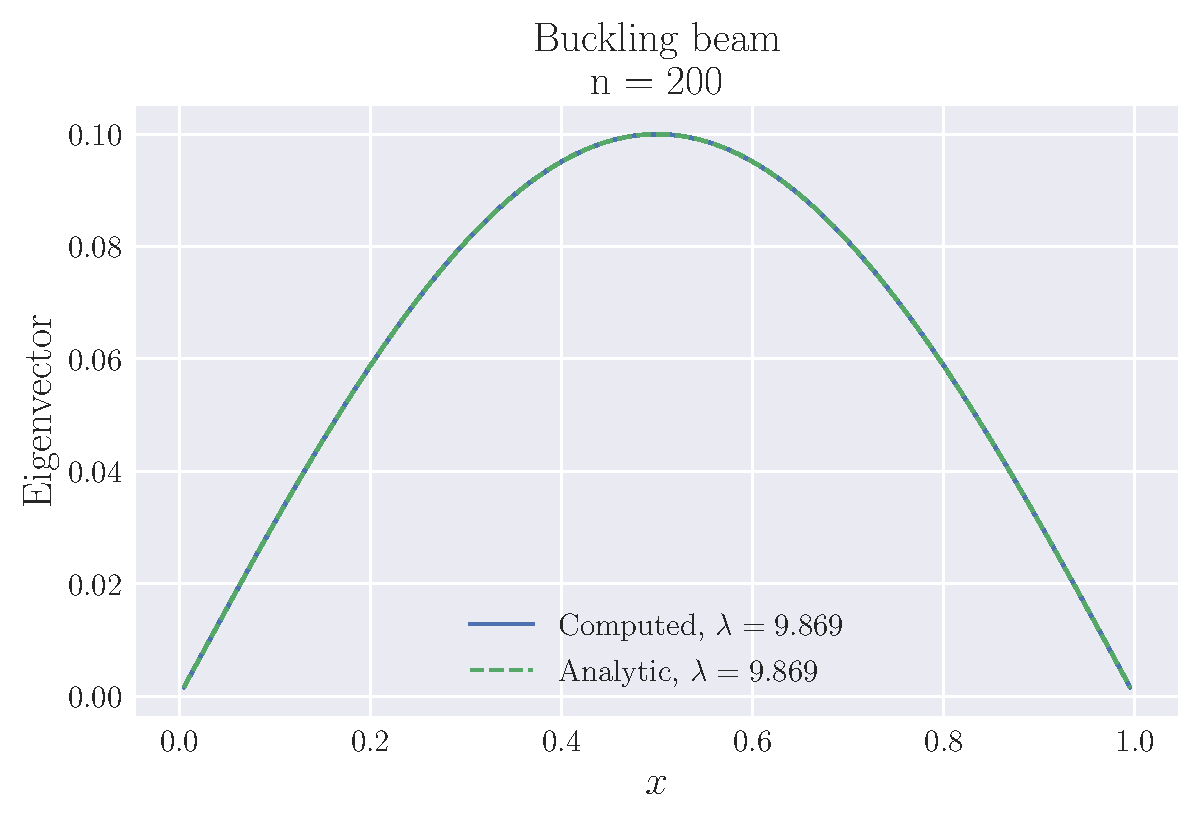
\includegraphics[width=\linewidth]{../output/BB_200_0.pdf}
	\label{fig:BB200}
	\caption{}
\end{figure}


\subsection{Unit-tests}

There are several sections in this code that can be tested independantly. We have developed tests for a general tridiagonal Toeplitz matrix that checks that the program finds the correct


\onecolumngrid
\begin{thebibliography}{}
\bibitem{lecnotes} http://compphysics.github.io/
ComputationalPhysics/doc/pub/eigvalues/html/.\_eigvalues-bs011.html
\bibitem{oppgavetekst} OPPGAVETEKST REF

\end{thebibliography}
\end{document}
